% PDFLatex


%%% presentation template
%%% daniel vogler, ETHZ
%%% davogler@ethz.ch


\documentclass[first,firstsupp,svgnames,9pt]{ethz_beamer}

\date{5 October 2017}
\email{\url{ davogler@ethz.ch}}
\meeting{Idaho National Laboratory}
%%%
%%%
%%%
%%% BEGIN DOCUMENT
%%%
%%%
%%%
%%%
\begin{document}
\beamertemplatenavigationsymbolsempty

%%%
%%% DEFINED COMMANDS
%%%
\newcommand{\fig}{./figures/}
\newcommand{\apause}{}%\pause}

%%%
%%% TITLEPAGE
%%%
\title{ {\begin{center} \LARGE Thermal Spallation Drilling \end{center}} }
\author[Daniel Vogler]{ \Large { \color{tangocolormediumskyblue}{D. Vogler} \inst{1,2}} S.D.C. Walsh \inst{3}, P. Rudolf von Rohr \inst{2}, M.O. Saar \inst{1} }
\institute{\small
  \inst{1} { {\color{tangocolormediumskyblue}{ETH Zurich}}, Geothermal Energy and Geofluids, Zurich, Switzerland}\\[5pt]
  \inst{2} { {\color{tangocolormediumskyblue}{ETH Zurich}}, Transport Processes and Reactions Laboratory, Zurich, Switzerland}\\[5pt]
  \inst{3} { {\color{tangocolormediumskyblue}{UNSW}}, School of Petroleum Engineering, Sydney, Australia}
  }

%%%
%%% SECTION BEHAVIOR
%%%
\setbeamertemplate{section in head/foot}{\hfill\insertsectionheadnumber.~\insertsectionhead}
\setbeamertemplate{section in head/foot shaded}{\color{structure!50}\hfill\insertsectionheadnumber.~\insertsectionhead}
\setbeamertemplate{section in toc}{\inserttocsectionnumber.~\inserttocsection}
% SECTION SLIDE
\AtBeginSection[] 
{{\usebackgroundtemplate[plain]{}
\begin{frame}<beamer>{Outline}
    \tableofcontents[currentsection,currentsubsection]
  \end{frame}   } }

%%%
%%% TITLEFRAME
%%%
\begin{frame}
  \Wider[5ex]{
  \maketitle
  \begin{center}
    \insertemail
  \end{center}
  }
\end{frame}

%%%
%%%
%%% INTRODUCTION
%%%
%%%
\section{Introduction}

%%% 
%%% ENERGY IN SWITZERLAND
%%%
\begin{frame}{Switzerland plans large-scale exploitation of \alert{deep geothermal energy}}
\Wider[1em]{
  \begin{itemize}
    \item Reservoir creation, from \alert{borehole drilling} to creation of \alert{heat exchanger}.\\[5pt]
    \item Capabilities to quantitatively \alert{model stimulation and reservoir operation}.\\[5pt]
    \item Advance process understanding and validation in \alert{underground lab experiments}. \\[5pt]
    \item Develop \alert{petrothermal P\&D project}.
  \end{itemize}
  \begin{figure}
    \begin{center}
	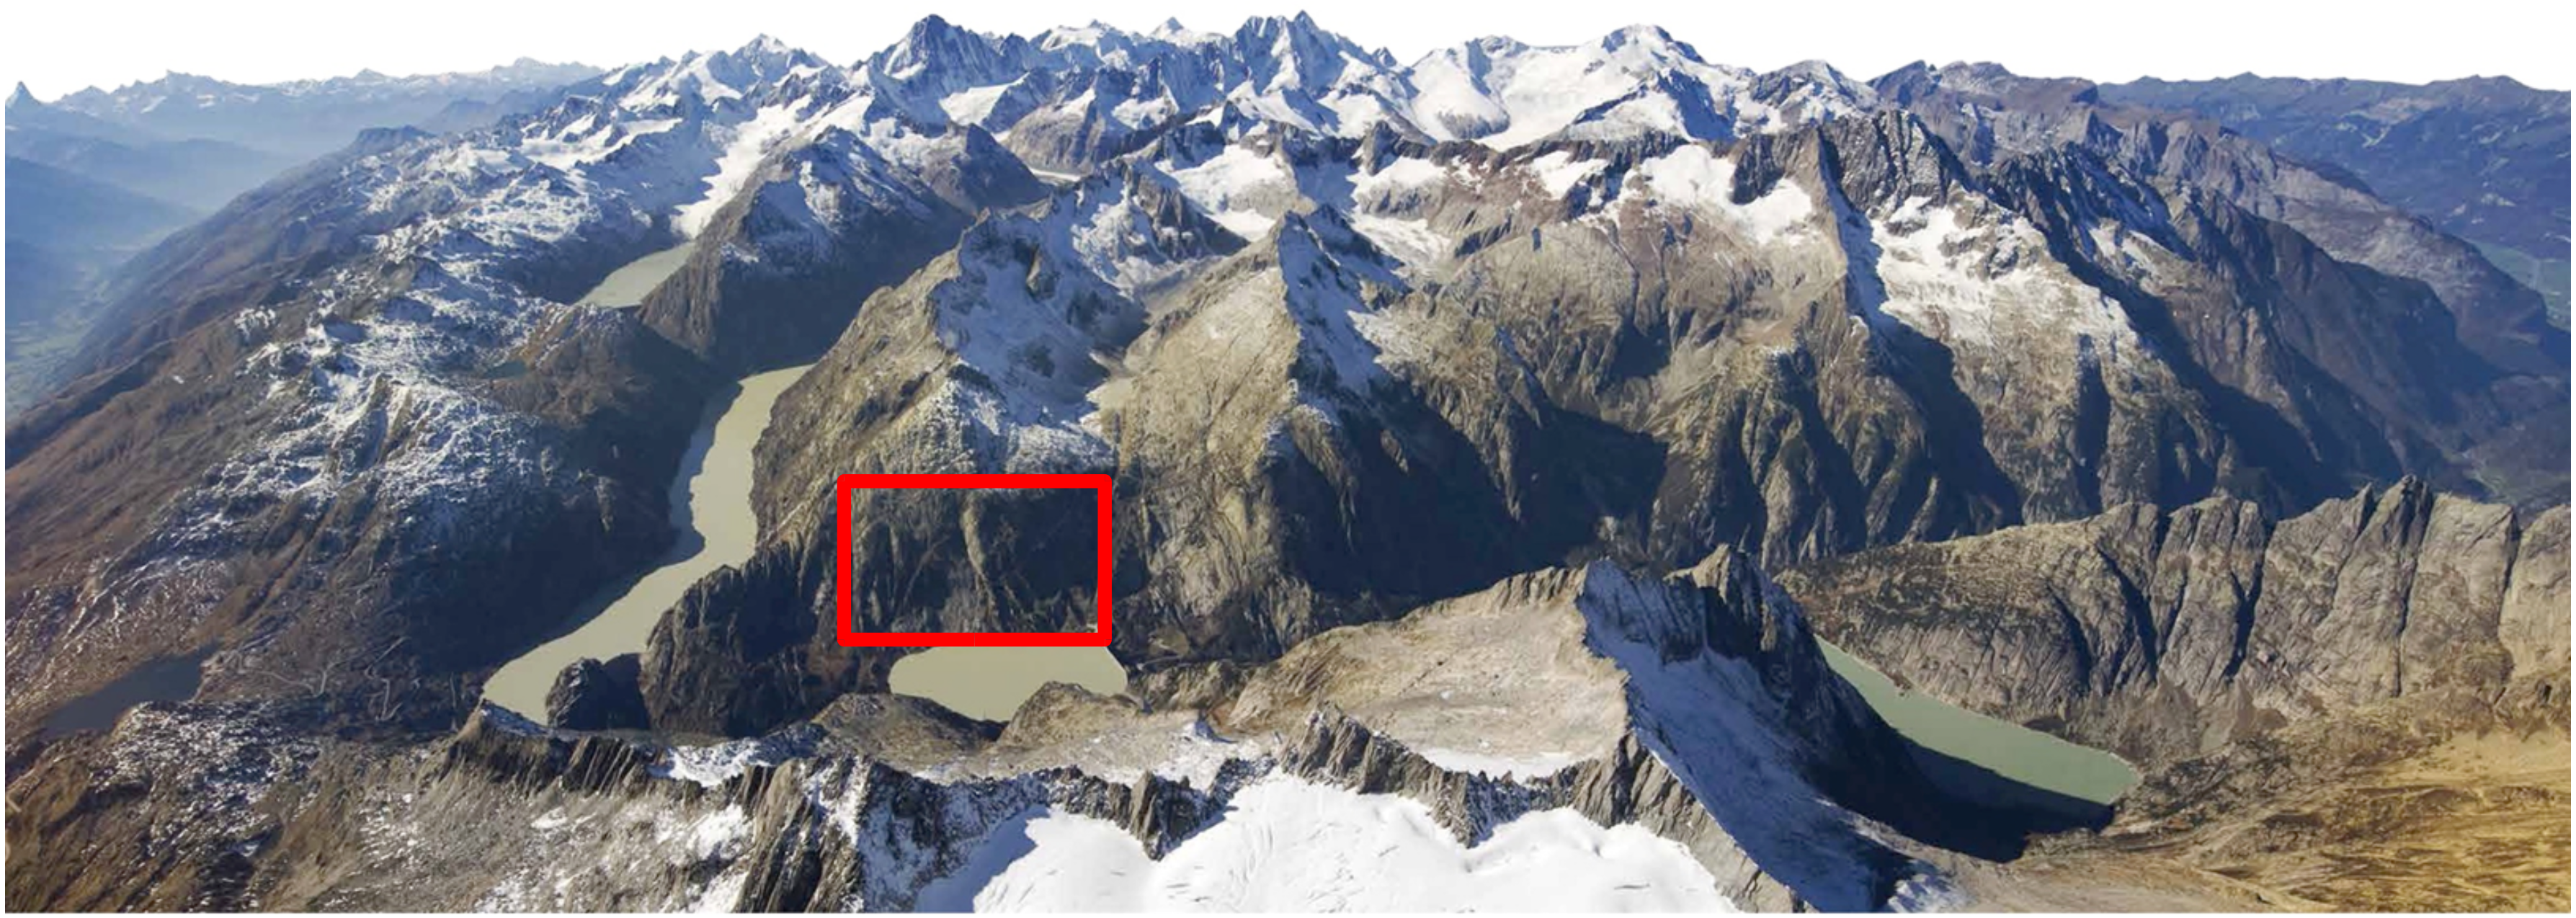
\includegraphics[width=0.95\linewidth]{./figures/grimsel_location_marked}
    \end{center}
    \caption{Grimsel Test Site (GTS) in the Swiss Alps.}
  \end{figure}
}
\end{frame}

%%%
%%% ROCKC PROPERTIES
%%%
\begin{frame}{Rock properties}
  \begin{figure}
    \begin{center}
      \includegraphics[height=0.28\linewidth]{\fig image_weathered_granite}
      \hfill
      \includegraphics[height=0.28\linewidth]{\fig image_granite}
      \hfill
      \includegraphics[height=0.28\linewidth]{\fig image_granodiorite}
      \caption{Mineral compositions of granitic rocks.}
    \end{center}
  \end{figure}
\end{frame}

%%%
%%% REFERENCES
%%%
\begin{frame}{References - MOOSE}
  \begin{enumerate}
    \item D. Gaston, C. Newman, G. Hansen, and D. Lebrun-Grandie. MOOSE: A parallel computational framework for coupled systems of nonlinear equations. Nucl. Engrg. Design, 239:1768–1778, 2009. \\[5pt]
    \item D.R. Gaston, J.W. Peterson, C.J. Permann, D. Andrš, A.E. Slaughter, and J.M. Miller. Continuous integration for concurrent computational framework and application development. Journal of Open Research Software, 2(1):1–6, July 2014. Special Collection: Working towards Sustainable Software for Science: Practice and Experiences, Article e10, http://dx.doi.org/10.5334/jors.as. \\[5pt]
    \item A. E. Slaughter, J.W.Peterson, D.R. Gaston, C.J.Permann, D. Andrš and J. M. Miller, "Continuous Integration for Concurrent MOOSE Framework and Application Development on GitHub," Journal of Open Research Software, pp. 1–4, Nov. 2015. Working towards Sustainable Software for Science: Practice and Experiences (WSSSPE2). \\[5pt]
    \item The MOOSE framework can be found here: \url{mooseframework.org}
  \end{enumerate}
\end{frame}

%%%
%%% FUNDING
%%%
\begin{frame}[c]{Funding}
  \begin{center}
    \includegraphics[width=0.6\textwidth]{\fig ethz_logo_black_transparent}\\[30pt]
    \includegraphics[width=0.47\textwidth]{\fig sccer_logo}
    \hfill
    \includegraphics[width=0.47\textwidth]{\fig logo-werner-siemens-stiftung}
  \end{center}
\end{frame}

%%%
%%% THANKS 1
%%%
\begin{frame}
\begin{center}
\alert{\Huge{Any Questions?}}
\vskip 0.5cm
-
\vskip 0.5cm
\large{\url{davogler@ethz.ch} }
\end{center}
\end{frame}

%%%
%%% TITLEFRAME
%%%
\begin{frame}
  \Wider[3ex]{
  \maketitle
  \begin{center}
    \insertemail
  \end{center}
  }
\end{frame}


\end{document}
